% L12c figure: two Q-networks. Each maps a state s to one Q-value per action.
%
% Top: the linear Q-network of the L12c example. The features phi_1(s), ...,
% phi_p(s) are fixed functions of the state (radial basis functions in the example),
% and only the weights W from the features to the Q-values are learned.
% Bottom: a deep Q-network, adapted from the DQN schematic of the eCornell AI in
% finance session 3 lecture (May 2026). Its hidden layers are learned as well.
%
% Drawn on November 6, 2026 with the palette and build of the L10c figures.
% The notebook SVG carries a dark palette added by theme_svg.py; keep new
% colors in that script's mapping when changing the palette here.
\documentclass[tikz,border=4pt]{standalone}
\usepackage[no-math]{fontspec}
\IfFontExistsTF{Arial}{\setsansfont{Arial}}{\setsansfont{TeX Gyre Heros}}
\renewcommand{\familydefault}{\sfdefault}
\usepackage{amsmath,amssymb}
\usetikzlibrary{arrows.meta, fit, backgrounds, calc, decorations.pathreplacing}

% Ink, blue, gray, and band match the L10c figures. Blue marks what is learned.
\definecolor{vnink}{HTML}{202124}
\definecolor{gdblue}{HTML}{0091FF}
\definecolor{gdgray}{HTML}{6D7278}
\definecolor{waband}{HTML}{EEF0F2}
\definecolor{netfill}{HTML}{E8F4FF}
\definecolor{nodefill}{HTML}{FFFFFF}

\begin{document}
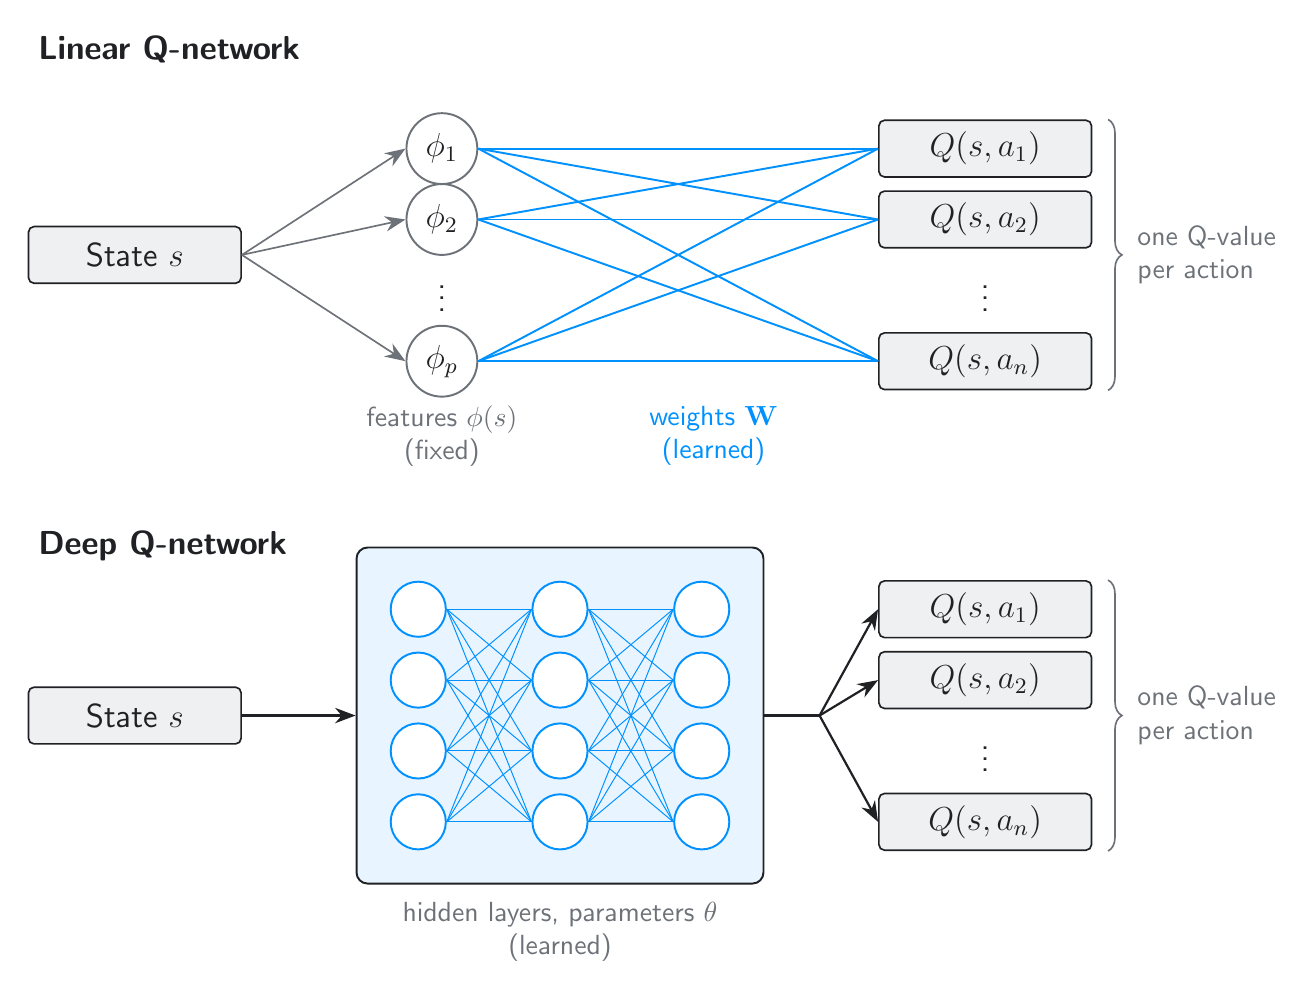
\begin{tikzpicture}[
  font=\sffamily\large,
  >={Stealth[length=2.6mm]},
  io/.style={draw=vnink, rounded corners=2pt, minimum width=2.7cm, minimum height=0.72cm,
    fill=waband, line width=0.6pt, text=vnink},
  feature/.style={circle, draw=gdgray, minimum size=9mm, inner sep=0pt, line width=0.7pt,
    fill=nodefill, text=vnink},
  neuron/.style={circle, draw=gdblue, minimum size=7mm, inner sep=0pt, line width=0.7pt,
    fill=nodefill},
  label/.style={font=\sffamily\normalsize, text=gdgray},
  title/.style={font=\sffamily\large\bfseries, text=vnink},
  fixed/.style={->, line width=0.6pt, draw=gdgray},
  weight/.style={line width=0.7pt, draw=gdblue},
  arrow/.style={->, line width=0.8pt, draw=vnink}
]

% ---------------------------------------------------------------- linear network
\node[title, anchor=west] at (-1.35, 1.25) {Linear Q-network};

\node[io] (s1) at (0, -1.35) {State $s$};

\node[feature] (f1) at (3.9,  0.00) {$\phi_{1}$};
\node[feature] (f2) at (3.9, -0.90) {$\phi_{2}$};
\node[text=vnink] (fd) at (3.9, -1.80) {$\vdots$};
\node[feature] (fp) at (3.9, -2.70) {$\phi_{p}$};
\node[label, align=center] at (3.9, -3.65) {features $\phi(s)$\\(fixed)};

\foreach \f in {f1, f2, fp} {
  \draw[fixed] (s1.east) -- (\f.west);
}

\node[io] (q1a) at (10.8,  0.00) {$Q(s, a_{1})$};
\node[io] (q2a) at (10.8, -0.90) {$Q(s, a_{2})$};
\node[text=vnink] (qda) at (10.8, -1.80) {$\vdots$};
\node[io] (qna) at (10.8, -2.70) {$Q(s, a_{n})$};

\foreach \f in {f1, f2, fp} {
  \foreach \q in {q1a, q2a, qna} {
    \draw[weight] (\f.east) -- (\q.west);
  }
}
\node[label, text=gdblue, align=center] at (7.35, -3.65) {weights $\mathbf{W}$\\(learned)};

% ------------------------------------------------------------------ deep network
\node[title, anchor=west] at (-1.35, -5.05) {Deep Q-network};

\node[io] (s2) at (0, -7.20) {State $s$};

\foreach \layer/\x in {1/3.6, 2/5.4, 3/7.2} {
  \foreach \i in {1,...,4} {
    \node[neuron] (h\layer-\i) at (\x, -5.85 - 0.9*\i + 0.9) {};
  }
}
\foreach \i in {1,...,4} {
  \foreach \j in {1,...,4} {
    \draw[line width=0.35pt, draw=gdblue] (h1-\i.east) -- (h2-\j.west);
    \draw[line width=0.35pt, draw=gdblue] (h2-\i.east) -- (h3-\j.west);
  }
}
\begin{scope}[on background layer]
  \node[draw=vnink, rounded corners=4pt, line width=0.7pt, fill=netfill,
    fit=(h1-1)(h1-4)(h3-1)(h3-4), inner sep=12pt] (network) {};
\end{scope}
\node[label, align=center] at (5.4, -9.95) {hidden layers, parameters $\theta$\\(learned)};

\draw[arrow] (s2.east) -- (s2.east -| network.west);

\node[io] (q1b) at (10.8, -5.85) {$Q(s, a_{1})$};
\node[io] (q2b) at (10.8, -6.75) {$Q(s, a_{2})$};
\node[text=vnink] (qdb) at (10.8, -7.65) {$\vdots$};
\node[io] (qnb) at (10.8, -8.55) {$Q(s, a_{n})$};

\coordinate (fan) at ($(network.east |- s2.east) + (0.7, 0)$);
\draw[line width=0.8pt, draw=vnink] (network.east |- s2.east) -- (fan);
\foreach \q in {q1b, q2b, qnb} {
  \draw[arrow] (fan) -- (\q.west);
}

% ------------------------------------------------------- one Q-value per action
\foreach \top/\bottom in {q1a/qna, q1b/qnb} {
  \draw[decorate, decoration={brace, amplitude=5pt}, line width=0.6pt, draw=gdgray]
    ($(\top.north east) + (0.2, 0)$) -- ($(\bottom.south east) + (0.2, 0)$)
    node[midway, right=7pt, label, align=left] {one Q-value\\per action};
}

\end{tikzpicture}
\end{document}
